% --------------------------------------------------------------
% This is all preamble stuff that you don't have to worry about.
% Head down to where it says "Start here"
% --------------------------------------------------------------
 
\documentclass[12pt]{article}
 
\usepackage[margin=1in]{geometry} 
\usepackage{amsmath,amsthm,amssymb}
\usepackage{enumerate}
\usepackage{graphicx}
\usepackage{pdfpages}
\usepackage{listings}
\graphicspath{{home/users/mark/Documents/school/math128a}}
 
\newcommand{\N}{\mathbb{N}}
\newcommand{\Z}{\mathbb{Z}}
\newcommand{\R}{\mathbb{R}}

 
\newenvironment{theorem}[2][Theorem]{\begin{trivlist}
\item[\hskip \labelsep {\bfseries #1}\hskip \labelsep {\bfseries #2.}]}{\end{trivlist}}
\newenvironment{lemma}[2][Lemma]{\begin{trivlist}
\item[\hskip \labelsep {\bfseries #1}\hskip \labelsep {\bfseries #2.}]}{\end{trivlist}}
\newenvironment{exercise}[2][Exercise]{\begin{trivlist}
\item[\hskip \labelsep {\bfseries #1}\hskip \labelsep {\bfseries #2.}]}{\end{trivlist}}
\newenvironment{reflection}[2][Reflection]{\begin{trivlist}
\item[\hskip \labelsep {\bfseries #1}\hskip \labelsep {\bfseries #2.}]}{\end{trivlist}}
\newenvironment{proposition}[2][Proposition]{\begin{trivlist}
\item[\hskip \labelsep {\bfseries #1}\hskip \labelsep {\bfseries #2.}]}{\end{trivlist}}
\newenvironment{corollary}[2][Corollary]{\begin{trivlist}
\item[\hskip \labelsep {\bfseries #1}\hskip \labelsep {\bfseries #2.}]}{\end{trivlist}}
 
\begin{document}
 
% --------------------------------------------------------------
%                         Start here
% --------------------------------------------------------------
 
%\renewcommand{\qedsymbol}{\filledbox}
 
\title{CMPS 242: HW3}%replace X with the appropriate number
\author{Mark Beers %replace with your name
} %if necessary, replace with your course title
 
\maketitle
 
\begin{enumerate}
	\item Linear Regression
	\begin{enumerate}[(a)]
		\item MLE estimation of $w, \beta$. Here we maximize the log likelihood. 
		\begin{align*}
		p(t|x, w, \beta) &= N(t|y(x,w), \beta^{-1}) \\
	w_{MLE}, \beta_{MLE}	&= \underset{w, \beta}{\operatorname{argmax}}\  log \prod_{i = 1}^{n} \frac{1}{\sqrt{2\pi \beta^{-1}}}exp\bigg(-\frac{(t_i - y(x_i, w))^2}{2\beta^{-1}}\bigg) \\
	&= \underset{w, \beta}{\operatorname{argmin}}\ -n\ log(\beta) + \beta \sum_{i=1}^{n} (t_i - y(x_i, w))^2
		\end{align*}
		Taking derivatives with respect to $w_0, w_1, w_2, w_3$, and setting equal to zero, we note that $\beta$ falls out of the equation in each case, giving us 4 equations and four unknowns. This means that our MLE estimates for $w$ won't depend on the variance $\beta^{-1}$ and they will take the standard form, 
		\begin{align*}
		X &= [1, x, x^2, x^3]\\
		w &= (X^T X)^{-1}X^T t
		\end{align*}
		Further, taking the derivative of the log likelihood with respect to $\beta$ yields the following. 
		\begin{align*}
		\frac{\partial}{\partial \beta}\bigg(\underset{w, \beta}{\operatorname{argmin}}\ -n\ log(\beta) &+ \beta \sum_{i=1}^{n} (t_i - y(x_i, w))^2\bigg) = 0 \\
		\implies \frac{n}{\beta_{MLE}} &=  \sum_{i=1}^{n} (t_i - y(x_i, w))^2 \\
		\implies \beta_{MLE}^{-1} &= \frac{1}{n}\sum_{i=1}^{n} (t_i - y(x_i, w_{MLE}))^2 
		\end{align*}
		Using this approach yields the following estimates for $w, \beta$ for 100, 1000, 10000 test points. 
		\begin{table}[htb]
			\begin{tabular}{|l|l|l|l|l|l|}
				\hline
				n training points & $w_0$     & $w_1$     & $w_2$     & $w_3$     & $\beta^{-1}$   \\ \hline
				100               & 0.2401381 & 2.0000394 & 0.9999990 & 2.9999995 & 0.8202118 \\ \hline
				1000              & 0.1834306 & 1.9981898 & 0.9999978 & 3.0000003 & 1.002905  \\ \hline
				10000             & 0.1903286 & 2.0004489 & 0.9999998 & 2.9999999 & 1.014826  \\ \hline
			\end{tabular}
		\end{table}
		We note that $w_1, w_2, w_3$ remain relatively constant while the intercept seems to get closer to the true value of $.2$. We also note that our estimate for the variance seems to improve once we get more than 100 training examples. 
		Interestingly, if we use the optimize module in scipy with method BFGS to perform this same task, optimizing over $\beta$ and $w$ simultaneously, we get very similar results for $w$, but $\beta$ is computed to be around $3.35$ in each case. I'm not certain why this would be. Also we note that accurate convergence of our minimization is very dependent on having a close starting value. 
		
		\item Repeat part a but with a fifth degree polynomial rather than a 3rd degree polynomial. This yields the following table of results using the mathematical approach above. We see that the MLE correctly sets $w_4, w_5$ to be very nearly 0. 
		
		
		\begin{table}[htb]
			\begin{tabular}{|l|l|l|l|l|l|l|l|}
				\hline
				n training points & $w_0$     & $w_1$    & $w_2$    & $w_3$     & $w_4$         & $w_5$         & $\beta^{-1}$ \\ \hline
				100               & .2224     & 2.0089   & 1.0000 & 2.99999 & -7.5716e-09 & 3.9693e-10  & 0.7998198  \\ \hline
				1000              & 0.14827 & 1.9964& 1.0000 & 3.0000 & -4.4164e-09 & -7.401052e-11 & 1.000897   \\ \hline
				10000             & .19577  & 2.0012 & .99999 & 3.0000  & 6.5339e-10  & 3.3887e-11  & 1.014  \\ \hline
			\end{tabular}
		\end{table}
		
		This time with the scipy approach we see similar but more extreme results. In particular, the coefficient estimates that we converge to seem even more dependent on the point we initialize the solver at. Often it will set $w_4, w_5$ to be small, but our estimates for $w_0,w_1, w_2, w_3$ can vary dramatically. 
		
		\item Bayesian Linear Regression \\
		In this problem we seek to maximize the following equation with respect to w and alpha, where $\beta=\alpha = 1$. 
		\begin{equation*}
		ln\ p(w|t) = -\frac{\beta}{2} \sum_{i=1}^{n} \bigg(t_i - w^T\phi(x_i)\bigg)^2 - \frac{\alpha}{2}w^Tw + const.
		\end{equation*}
		From the book we note that the posterior distribution is as follows.
		\begin{align*}
		p(w|t) &= N(w|m_N, S_N) \\
		m_N &= \beta S_N\Phi^Tt \\
		S_N^{-1} &= \alpha I + \beta \Phi^t\Phi \\
		\implies m_N &= (I + \Phi^t\Phi)^{-1}\Phi^T t
		\end{align*}
		This equation will give us the MLE's for w that we need. The results are summarized in the following tables below. Some plots of the estimated curves are also provided.
		
		\begin{table}[htb]
			\centering
			\begin{tabular}{|l|l|l|l|l|}
				\hline
				Training Examples & $w_0$     & $w_1$     & $w_2$     & $w_3$     \\ \hline
				100               & 0.2345511 & 1.9999760 & 0.9999999 & 2.9999995 \\ \hline
				1000              & 0.1830405 & 1.9981858 & 0.9999979 & 3.0000003 \\ \hline
				10000             & 0.1902861 & 2.0004486 & 0.9999999 & 2.9999999 \\ \hline
				True & 0.2 & 2 & 1 & 3 \\ \hline
			\end{tabular}
			\caption{Cubic Polynomial Fit Coefficient Results} \label{tab:sometab}
		\end{table}
	
		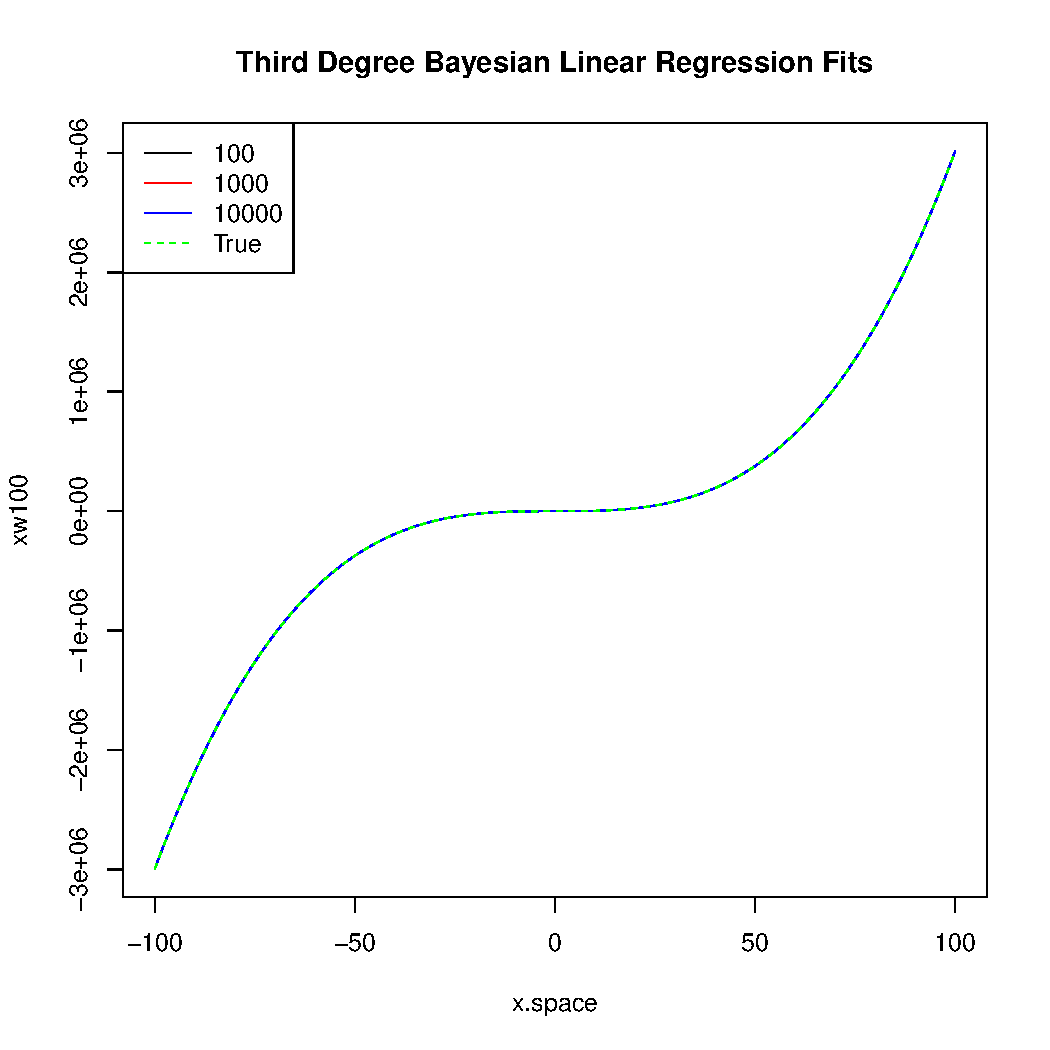
\includegraphics[scale=.5]{third_degree_bayesian_fits.pdf}
	
		As we can see looking at the table of coefficients and at the plot of Third Degree Bayesian Regression fits, the bayesian regression approach gives very accurate results, with all curves lining up almost identically. The fifth degree polynomial fits worked fairly well also. Unfortunately however, I was unable to invert the matrix $(I + \Phi^T\Phi)$ and so a numerical minimization approach had to be used. The results from this approach are still graphically good, though we note in the table that the coefficient estimates are much less exact than with the third degree bayesian regression. 
		
		
		\begin{table}[htb]
			\centering
			\begin{tabular}{|l|l|l|l|l|l|l|}
				\hline
				Training Examples & $w_0$     & $w_1$  & $w_2$   & $w_3$   & $w_4$     & $w_5$      \\ \hline
				100               & -2033.495 & -5.526 & 2.00095 & 3.004   & -9.549e-5 & -3.5633e-7 \\ \hline
				1000              & 80.921    & -8.63  & .9738   & 3.00479 & 2.156e-6  & -4.219e-7  \\ \hline
				10000             & -6.157    & -8.849 & 1.004   & 3.005   & -4.489e-7 & -4.5357e-7 \\ \hline
				True             & 0.2    & 2 & 1    & 3   & 0 & 0 \\ \hline
			\end{tabular}
			\caption{Quintic Polynomial Fit Coefficient Results} \label{tab:sometab}
		\end{table}
		
		 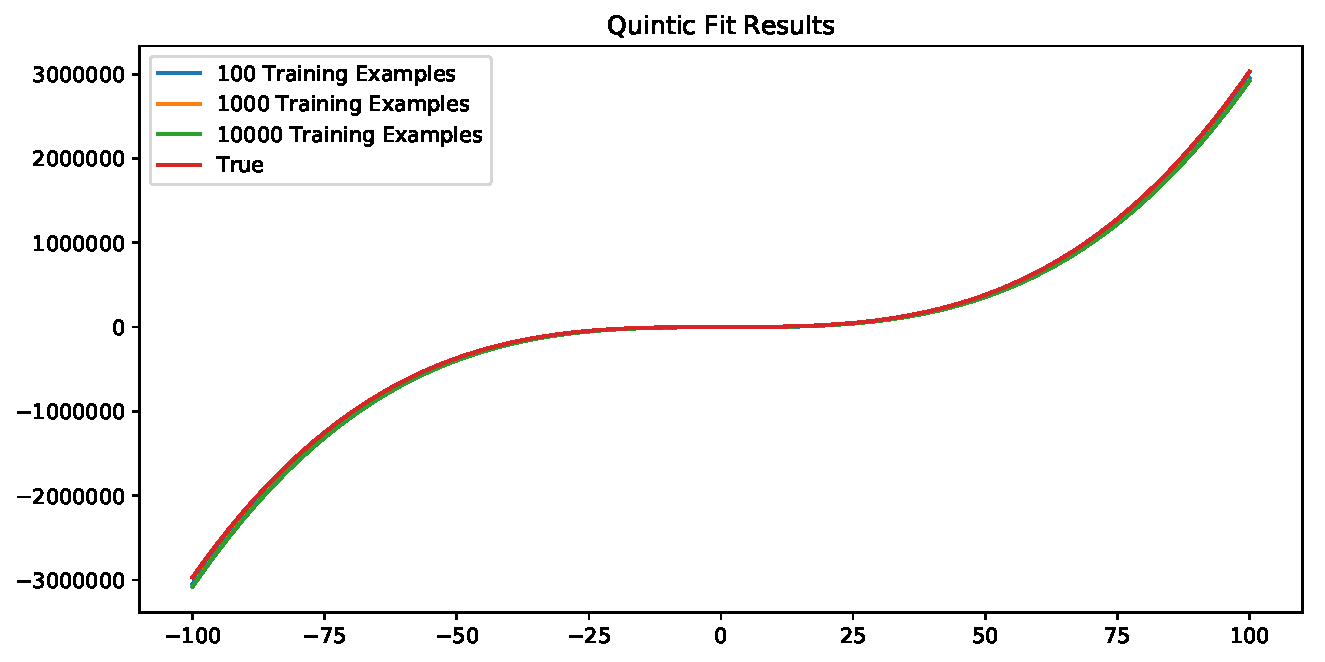
\includegraphics[scale=.65]{quintic_fit.pdf}
		
		
	\end{enumerate}
	
\item Naive Bayes Text Classification \\
In this problem, we perform text classification with a Naive Bayes Classifier. We're given 12 datasets, Enron1.ham, Enron2.ham, ... Enron6.ham, Enron1.spam, Enron2.spam, ..., Enron6.spam. We use Enron1 through Enron5 to train a  classifier to differentiate between ham and spam, and test on Enron6. We classify as ham if: 
\begin{align*}
P(ham|data) &> P(spam|data) \\
\implies \frac{P(data|ham)P(ham)}{P(data)} &> \frac{P(data|spam)P(spam)}{P(data)} \\
\implies P(data|ham)P(ham) &> P(data|spam)P(spam) \\
P(ham) &= \frac{15045}{15045 + 12669}\\
P(spam) &= 1 - P(ham) \\
P(data|ham) &= \prod_{n = 1}^{N} P(\text{test example word n}|ham)\\
P(data|spam) &= \prod_{n = 1}^{N} P(\text{test example word n}|spam)
\end{align*} 
In the above equations N indicates the number of words in a given test email. Different prior probabilities arising from different numbers of spam and ham emails in the training set are accounted for in the above equations. For computational reasons, all calculations are done on the log scale. Further, all computations are done without the use of python packages like sklearn. Below we report accuracy results for versions with and without laplace smoothing. Accuracy is measured as the proportion of emails in the Enron6 dataset that are classified correctly.


\begin{table}[htb]
	\centering
	\begin{tabular}{|l|l|l|l|}
		\hline
		Smoothing & Ham Accuracy        & Spam Accuracy       & Total Accuracy                   \\ \hline
		None      & $973/1500$  & $3274/4499$ & $4247/5999 \simeq 0.708$ \\ \hline
		Laplace   & $1431/1500$ & $4465/4499$ & $5896/5999 \simeq 0.983$ \\ \hline
	\end{tabular}
	\caption{Naive Bayes Classifier Accuracy Results} \label{tab:sometab}
\end{table}

As we can see in the table above, adding laplace smoothing dramatically improves accuracy. This can  in large part be explained by a large issue that arises when laplace smoothing isn't included. Namely, if laplace smoothing isn't implemented, we will inevitably encounter words in the test data that aren't included in the training data. In this situation the Niave Bayes classifier without laplace smoothing will set the probability of that particular word given a certain class to zero. After a log transformation, we're left with a $P(class|data) = -\infty$. If both class's training sets don't include a word in the test email, then we're left with $P(class\ 0|data) = P(class\ 1|data) = -\infty$. In this situation, I assigned that email to the ham class with probability equal to the ham prior. A more sophisticated approach involving ignoring the word not existent in the training set would probably perform better. We also chose to not do anything special with punctuation. It would be interesting to see if removing punctuation improved the performance of the classifier. Below we include a list of the most discriminative words based on the learned probabilities. In order to get this table, we compute the log probability associated with each word for spam and ham, and then find the absolute value of the difference between these two log probabilities. Sorting on this difference gives us table four. 

\begin{table}[htb]
	\centering
	\begin{tabular}{|l|l|}
		\hline
		Word      & abs(log probability difference) \\ \hline
		enron     & 10.411474                       \\ \hline
		kaminski  & 7.968558                        \\ \hline
		dynegy    & 7.958526                        \\ \hline
		pills     & 7.898633                        \\ \hline
		viagra    & 7.810160                        \\ \hline
		ect       & 7.561901                        \\ \hline
		computron & 7.483230                        \\ \hline
	\end{tabular}
	\caption{Most Discriminative Words} \label{tab:sometab}
\end{table}
 
\end{enumerate}


\end{document}